\section{Results}
\label{sec:results}

We report $\dNE$ against \textsc{Wait} --- negative means better than the admissible status
quo --- in Table~\ref{tab:delta} cell by cell, and in Fig.~\ref{fig:delta} against capacity.

\begin{table}[t]
\centering
\caption{$\dNE$ at $v=1$\,d; negative favours the first arm. \textbf{Bold} marks significance at
Holm-corrected $\alpha=0.05$ over the \nContrast{} cells of each contrast. Five seeds per cell,
paired.}
\label{tab:delta}
\small
\begin{tabular}{@{}llrrrrr@{}}
\toprule
Contrast & $o$ & A0 & A1 & A2 & A3 & A4\\
\midrule
\textsc{Correct-Distill} $-$ \textsc{Wait} & 5\,min & \textbf{-0.0070} & \textbf{-0.0074} & -0.0024 & -0.0005 & -0.0015\\
 & 30\,min & \textbf{-0.0087} & \textbf{-0.0090} & \textbf{-0.0043} & -0.0014 & \textbf{-0.0057}\\
 & 90\,min & \textbf{-0.0096} & \textbf{-0.0083} & \textbf{-0.0044} & \textbf{-0.0012} & -0.0003\\
\addlinespace
\textsc{Distill-Only} $-$ \textsc{Wait} & 5\,min & \textbf{-0.0018} & \textbf{-0.0030} & \textbf{+0.0023} & \textbf{+0.0057} & \textbf{+0.0056}\\
 & 30\,min & \textbf{-0.0027} & \textbf{-0.0039} & \textbf{+0.0020} & \textbf{+0.0094} & \textbf{+0.0052}\\
 & 90\,min & \textbf{-0.0039} & \textbf{-0.0041} & \textbf{+0.0015} & \textbf{+0.0091} & \textbf{+0.0051}\\
\addlinespace
\textsc{Correct-Distill} $-$ \textsc{Distill-Only} & 5\,min & \textbf{-0.0052} & \textbf{-0.0044} & \textbf{-0.0047} & \textbf{-0.0063} & \textbf{-0.0071}\\
 & 30\,min & \textbf{-0.0060} & \textbf{-0.0050} & \textbf{-0.0064} & \textbf{-0.0108} & \textbf{-0.0108}\\
 & 90\,min & \textbf{-0.0057} & \textbf{-0.0042} & \textbf{-0.0059} & \textbf{-0.0103} & \textbf{-0.0054}\\
\addlinespace
\bottomrule
\end{tabular}

\end{table}

\begin{figure}[t]
\centering
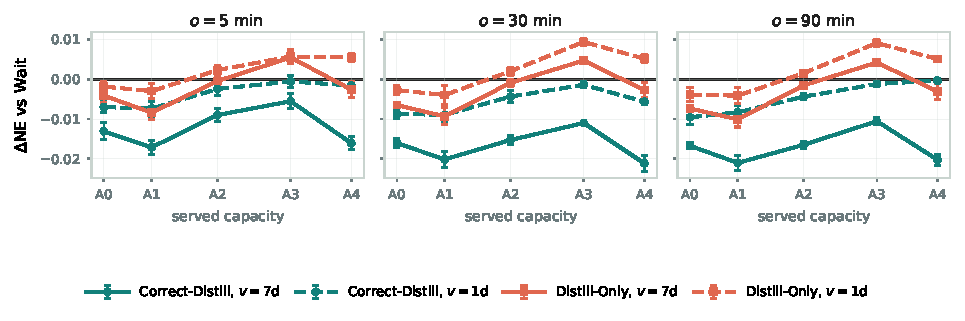
\includegraphics[width=\textwidth]{figs/delta}
\caption{$\dNE$ against \textsc{Wait} across the capacity ladder, one panel per write delay;
below the line is better than waiting. \textsc{Correct-Distill} is below it everywhere and
\textsc{Ulc} tracks it closely. \textsc{Distill-Only} crosses the line between A1 and A2 at
every $o$. The frozen teacher matches the live one at $o=30$ and $90$ and separates from it at
$o=5$ for the larger students. Bars are the standard deviation of the five per-seed
differences.}
\label{fig:delta}
\end{figure}

\paragraph{The censored label is expensive; waiting is not a straw man.}
\textsc{Wait} beats \textsc{Fresh} by \waitFreshFive{} $\NE$ on average at $o=5$ minutes,
falling to \waitFreshNinety{} at $o=90$ --- an ordering that follows $F(o)$, since the censored
label is wrong for a $1-F(o)$ share of eventual positives. This fixes the scale: the
differences discussed next are one to two orders of magnitude smaller than the cost of getting
the label wrong outright.

\paragraph{The hybrid target improves on waiting.}
\textsc{Correct-Distill} has lower $\NE$ than \textsc{Wait} in all \cdWaitN{} cells,
\cdWaitSig{} of them significantly, with gains from \cdWaitMax{} to \cdWaitMin{}. The gain is
largest where the served model is smallest and shrinks as capacity grows: averaged over write
delays it is \cdWaitSmallest{} at A0 and \cdWaitLargest{} at A4.

That decay is expected, but it bounds the claim. The teacher is fixed at \teacherParams{}
parameters --- three orders of magnitude larger than the student at A0, comparable at A4 --- so
part of the small-capacity gain is the teacher's capacity delivered at no serving cost, which
is what distillation is for, rather than anything specific to delayed feedback. What survives
at A4, where student and teacher are the same size and the gain is still negative in all three
cells, is the delayed-feedback component.

\paragraph{Removing the hard label does not.}
\textsc{Distill-Only}, our most informative result, beats \textsc{Wait} at the two smallest
capacities (\doWaitSmall{} on average) and \emph{loses}
to it at the three largest (\doWaitLarge{}), crossing over between A1 and A2 at every write
delay (Fig.~\ref{fig:delta}). All \doWaitSig{} cells are significant, so the crossing is not
noise.

The reading we find most plausible is that a purely soft target acts as a regulariser, whose
benefit is a variance reduction that a low-capacity model can use and a higher-capacity one no
longer needs~\cite{menon2021statistical}: at \capMin{} parameters the model cannot exploit the
hard label's extra information and gains from a smoother target, while by A2 it can, and
discarding the realised outcome throws away signal it could now use. Against
\textsc{Correct-Distill} the comparison is unambiguous: the hybrid wins all \cdDoSig{} cells by
\cdDoMean{} on average, so keeping the observed positive and softening only the negatives is
strictly the better construction.

This cuts against the motivation of Sect.~\ref{sec:allinone} rather than for it: a record
carrying no hard label is the most convenient object for a multi-objective pipeline, and it is
exactly the one that costs accuracy once the model is large enough to matter.

\paragraph{Parity with the online corrector.}
\textsc{Correct-Distill} and \textsc{Ulc} share Eq.~\eqref{eq:hybrid} and differ only in how $w$
is estimated. They are near-indistinguishable: mean $\dNE$ \cdUlcMean{}, with \cdUlcNs{} of \cdUlcN{} cells
showing no significant difference. In the \cdUlcSigN{} cells that do differ, \textsc{Ulc} is the
better of the two, by at most \cdUlcSigMax{}. Plainly: \emph{the offline teacher does not beat
the online corrector}. Any case for the teacher route rests on what it does to the pipeline
(Sect.~\ref{sec:allinone}), not on the metric.

\paragraph{How much of the teacher must stay live.}
Our default teacher keeps learning from the matured stream: a service, not an artifact.
Re-running \textsc{Correct-Distill} with it frozen after causal initialisation, so that it never
sees a matured record during the streaming period, costs \frzMean{} $\NE$ on average
(\frzSig{} of \nContrast{} cells significant). The
average hides the structure that matters. At $o=90$ minutes freezing is free --- the frozen
teacher is in fact marginally \emph{better}, \frzNinety{} --- and at $o=30$ it is nearly so. The
cost concentrates in the hardest corner: at $o=5$ minutes and the two largest capacities it
reaches \frzFiveLarge{}. Frozen \textsc{Correct-Distill} still beats \textsc{Wait} in
\frzWaitBeat{} of \frzWaitN{} cells, failing only at $o=5$ with a large student.

The teacher can therefore be a build-time artifact rather than a running service for most of
the grid, which is the cheaper operating point; it has to stay live exactly where the pipeline
is freshest and the model largest, because that is where its own initialisation goes stale
fastest relative to what the student could otherwise learn.

\paragraph{Distance to the ceiling.}
For scale, \textsc{Oracle} --- which labels the fresh record with an outcome that has not
happened --- is better than \textsc{Correct-Distill} in \cdOracleBeat{} of \cdOracleN{} cells,
by \cdOracleMean{} on average. The hybrid target therefore recovers much but not all of what
perfect foresight would be worth, and the residual grows with capacity.
